\subsection*{Teil C: Winkelbeziehungen (25 Minuten)}

\begin{merkbox}[Wichtige Winkelarten]
    \textbf{Nebenwinkel:} Ergänzen sich zu 180°\\
    \textbf{Scheitelwinkel:} Sind gleich groß\\
    \textbf{Stufenwinkel:} An parallelen Geraden gleich groß\\
    \textbf{Wechselwinkel:} An parallelen Geraden gleich groß
\end{merkbox}

\begin{enumerate}[label=\arabic*., resume]

    \item \textbf{Bestimme die fehlenden Winkel:}

    \vspace{0.5cm}

    \begin{center}
        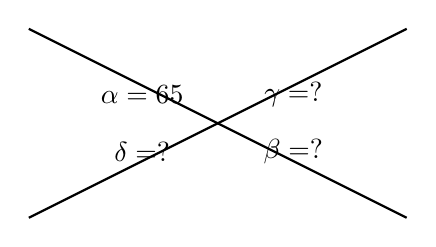
\begin{tikzpicture}[scale=1.2]
            % Sich kreuzende Geraden
            \draw[thick] (-2,-1) -- (2,1);
            \draw[thick] (-2,1) -- (2,-1);

            % Winkel markieren
            \node at (-0.8,0.3) {$\alpha = 65°$};
            \node at (0.8,-0.3) {$\beta = ?$};
            \node at (0.8,0.3) {$\gamma = ?$};
            \node at (-0.8,-0.3) {$\delta = ?$};
        \end{tikzpicture}
    \end{center}

    $\beta = $ \underline{\hspace{2cm}} (weil \underline{\hspace{4cm}})

    $\gamma = $ \underline{\hspace{2cm}} (weil \underline{\hspace{4cm}})

    $\delta = $ \underline{\hspace{2cm}} (weil \underline{\hspace{4cm}})

    \vspace{1cm}

    \item \textbf{Parallele Geraden und Winkel:}

    \vspace{0.5cm}

    \begin{center}
        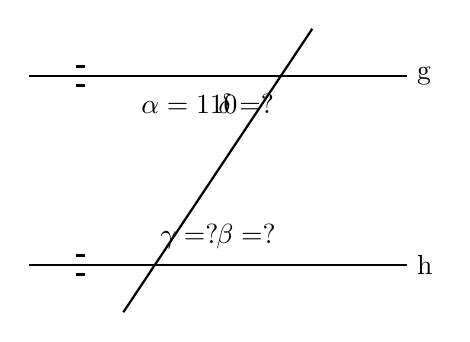
\begin{tikzpicture}[scale=1.2]
            % Parallele Geraden
            \draw[thick] (-2,1) -- (2,1) node[right] {g};
            \draw[thick] (-2,-1) -- (2,-1) node[right] {h};
            \draw[thick] (-1,-1.5) -- (1,1.5);

            % Winkel markieren  
            \node at (-0.3,0.7) {$\alpha = 110°$};
            \node at (0.3,-0.7) {$\beta = ?$};
            \node at (-0.3,-0.7) {$\gamma = ?$};
            \node at (0.3,0.7) {$\delta = ?$};

            % Parallele Zeichen
            \draw[thick] (-1.5,0.9) -- (-1.4,0.9);
            \draw[thick] (-1.5,1.1) -- (-1.4,1.1);
            \draw[thick] (-1.5,-0.9) -- (-1.4,-0.9);
            \draw[thick] (-1.5,-1.1) -- (-1.4,-1.1);
        \end{tikzpicture}
    \end{center}

    Die Geraden g und h sind parallel.

    $\beta = $ \underline{\hspace{2cm}} (weil \underline{\hspace{4cm}})

    $\gamma = $ \underline{\hspace{2cm}} (weil \underline{\hspace{4cm}})

    $\delta = $ \underline{\hspace{2cm}} (weil \underline{\hspace{4cm}})

    \vspace{1cm}

    \item \textbf{Anwendungsaufgabe:}

    Ein Verkehrsschild steht schief. Der Winkel zwischen dem Pfahl und dem Boden beträgt 85°. 

    \vspace{0.5cm}

    \begin{center}
        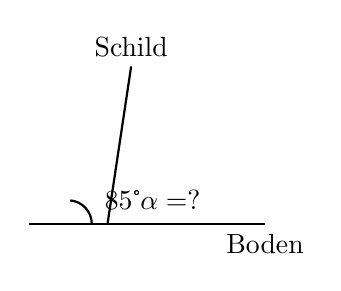
\begin{tikzpicture}[scale=1]
            \draw[thick] (0,0) -- (3,0) node[below] {Boden};
            \draw[thick] (1,0) -- (1.3,2) node[above] {Schild};
            \draw[thick] (0.8,0) arc (0:85:0.3);
            \node at (1.2,0.3) {85°};
            \node at (1.8,0.3) {$\alpha = ?$};
        \end{tikzpicture}
    \end{center}

    Wie groß ist der Winkel $\alpha$ zwischen Schild und Boden?

    $\alpha = $ \underline{\hspace{3cm}}

    \textit{Begründung:} \underline{\hspace{6cm}}

\end{enumerate}